\begin{XeClass}{GlobExpander}
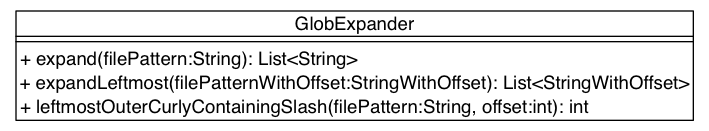
\includegraphics[width=10cm]{cdig/GlobExpander.png}
    
    \begin{XeMethod}{\XePublic}{List<String>}{expand}
         
 静态方法expand()匹配指定模式的文件名或目录名称filePattern
 并将其结果存入List<String>对象fullyExpanded中返回

    \end{XeMethod}

    \begin{XeMethod}{\XePrivate}{List<StringWithOffset>}{expandLeftmost}
         
 静态方法expandLeftmost()最左匹配带有偏移量模式的文件名或目录名称filePatternWithOffset
 从内部类StringWithOffset对象filePatternWithOffset中获得filePattern
 并调用leftmostOuterCurlyContainingSlash(filePattern,ilePatternWithOffset.offset)方法
 获得leftmost值,若为-1则返回null
 通过给定的leftmost获得filePattern的子串赋值为prefix
 以leftmost整数值作为起点遍历filePattern串中的字符,
 并以'//','{','}',','分情况处理

    \end{XeMethod}

    \begin{XeMethod}{\XePrivate}{int}{leftmostOuterCurlyContainingSlash}
         
 静态方法leftmostOuterCurlyContainingSlash以offset整数值作为起点遍历filePattern串中的字符
 并以'//','{','}','/'分情况处理,找到能在'{}'字符之间找到'/'的最大下标值并返回
 找不到结果则返回-1

    \end{XeMethod}


\end{XeClass}
